\problemname{Klockan}
Om någon frågar hur mycket klockan är, svarar de flesta ``kvart över fem'', \texttt{15:29} eller något liknande.
Vill man göra det lite svårare så kan man annars svara med vinkeln mellan tim- och minutvisaren, eftersom man ur denna information entydigt kan bestämma klockslaget.
Dock är det många människor som är ovana vid detta sätt att ange tider, så det vore bra att ha ett datorprogram som översätter till ett mer normalt format.
Du ska skriva ett sådant program.

\begin{figure}[h]
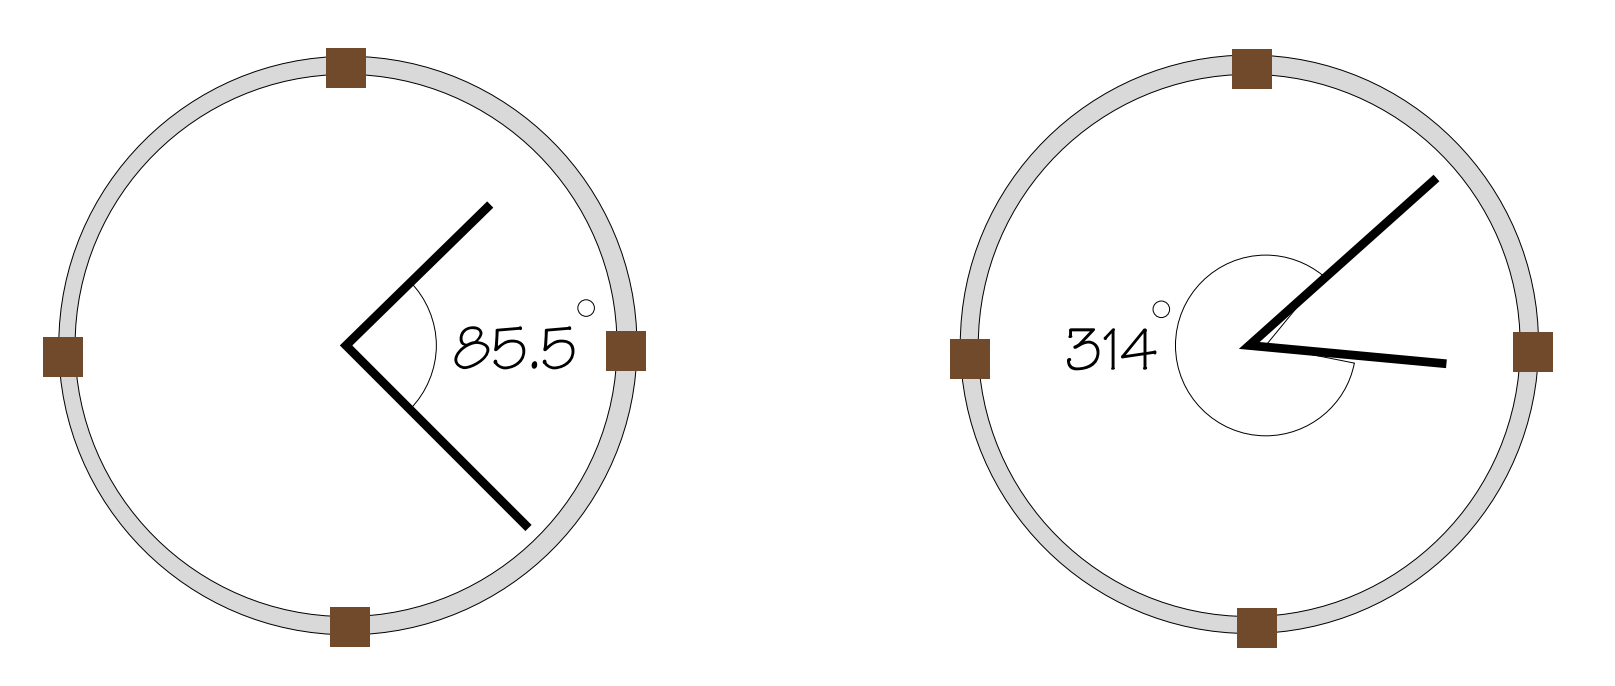
\includegraphics[width=\textwidth]{fig.png}
    \caption{Klockan till vänster är \texttt{01:21} och den till höger är \texttt{03:08}.}
\end{figure}

Vi förutsätter att vår klocka saknar sekundvisare och endast visar ett helt antal minuter (det vill säga: båda visarna hoppar framåt bara på hel minut).
Vinkeln avläses genom att utgå från timvisaren och sedan mäta hur många grader medurs minutvisaren ligger (se figuren).
För att undvika decimaler anges vinkeln i tiondels grader (så att $85.5$ grader skrivs som $855$).
Detta tal är alltid ett heltal mellan $0$ och $3595$ (inklusive) och är, som en följd av att endast hela minuter visas, alltid delbart med $5$.

\section*{Indata}
Indatan består av ett enda heltal mellan $0$ och $3595$ -- vinkel mellan de två visarna, i tiondels grader.

\section*{Utdata}
Skriv ut det klockslag som vinkeln motsvarar, på formatet \texttt{hh:mm}.
Om antalet timmar är ensiffrigt ska du ändå skriva ut en ledande nolla i svaret.
Vi förutsätter att det är morgon, så alla tider ska dessutom ligga mellan \texttt{00:00} och \texttt{11:59} (inklusive).

\section*{Poängsättning}
Din lösning kommer att testas på tre olika testfall.
De två första testfallen ger $33$ poäng vardera, medan det sista ger $34$ poäng.
